\documentclass[../main.tex]{subfiles}
\begin{document}
\chapter{Rigid Bodies}
Rigid body problems are a class of $N$-body problems where distances between the $N$ particles are fixed:
\[
  |\vec{x}_i - \vec{x}_j| = \text{constant}
\]
These are often tractable problems and usually arise due to very strong internal forces between particles.
Such a system of particles is known as a \textit{rigid body}.

The only motions a rigid body can experience are \textbf{translations of the centre of mass}, which we covered in \cref{systemsOfParticles}, and \textbf{rotations}, which we will cover now.
\section{Angular Velocity}
In three dimensions, rotations are described by a vector quantity $\vec{\omega}$ called the \textit{angular velocity}.
\begin{definition}[Angular Velocity]
  The \textit{angular velocity} $\vec{\omega}$ is defined as:
  \[
    \vec{\omega} = \omega \uvec{n}
  \]
  where $\uvec{n}$ points along the axis of rotation and $\omega = |\vec{\omega}| = \dot{\theta}$ is the angular speed of rotation.
\end{definition}
\begin{remark}[Right Hand Rule]
  We define $\uvec{n}$ so that it always points in the direction where if you align you right hand thumb along the positive direction of the axis of rotation, the rotation is in the direction that your fingers curl.
\end{remark}
The key equation for rotations is:
\begin{equation}
  \dot{\vec{x}} = \vec{\omega} \times \vec{x} \label{angularVelocityCross}
\end{equation}
This can be seen in the following diagram:
\begin{center}
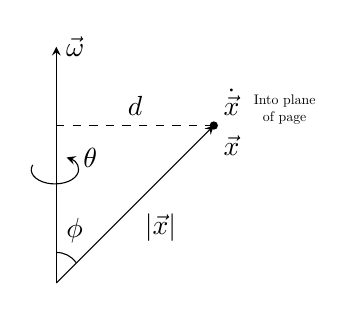
\begin{tikzpicture}[>=stealth]
  \draw[->] (0, 0)  -- (0, 3) node[right] {$\vec{\omega}$};
  \draw[->] (0, 0) -- (2, 2) node[below right] {$\vec{x}$} node[midway, below right] {$|\vec{x}|$};
  \fill (2, 2) circle (1.5pt) node[above right] {$\dot{\vec{x}}$};
  \node[text width=2cm, align=center, scale=0.5] at (2.9, 2.2) {Into plane of page};
  \draw[dashed] (2, 2) -- (0, 2) node[midway, above] {$d$};
  \draw[->, yscale=0.6] (-0.3,2.5) arc [start angle=-200,end angle=60,radius=0.3] node[xshift=0.3cm] {$\theta$};
  \draw (0.25,0.26) arc [start angle=35,end angle=90,radius=0.3] node[above right] {$\phi$};
\end{tikzpicture}
\end{center}
$\dot{\vec{x}}$ is orthogonal to both $\vec{\omega}$ and $\vec{x}$ and acts \textbf{into the plane of the page} in the above diagram.

The magnitude of $\uvec{n} \times \vec{x}$ is the distance between $\vec{x}$ and the axis of rotation:
\[
  |\uvec{n} \times \vec{x}| = |\uvec{n}||\vec{x}|\sin \phi = d
\]
and so:
\[
  |\dot{\vec{x}}| = \omega|\uvec{n} \times \vec{x}| = \omega d
\]
Therefore, the particle has speed $\omega d$, so $|\dot{\theta}| = \omega$

In addition to the angular velocity, a rotation must also specify a point about which the axis of rotation passes through.
For example, if we specify that the axis of rotation is the $z$-axis, then this does \textbf{not} specify the rotation as we do not know where the object is relative to this axis.
In the diagram, the vector $\vec{x}$ is measured from a point on the axis and we could have taken any point on the axis and it would be the same rotation.
The upshot of this is that in \cref{angularVelocityCross}, $\vec{x}$ must be relative to some arbitrary point on the axis of rotation.
\section{Moment of Inertia}
Continued next lecture.
\end{document}
